
\section{Solution}
\label{sec:auswertung}

\subsection{Aufgabe 1} 


Es wird eine Monte-Carlo-Simulation eines einzelnen Spins durchgeführt.
Dabei wird die Magnetisierung $m$ jeweils in Abhängigkeit des externen Magnetfeldes $H \in [-5,5] $ bestimmt.
Es werden $10^5$ Schritte durchgeführt.
Die Ergebisse und die Abweichung zum analytischen Ergebis sind in den folgenden Abbildungen dargestellt.
Es ist zu erkennen, dass die Abweichung ansteigt, wenn das externe Feld sich der $0$ nähert. 
Das könnte an dem numerischen Rauschen liegen, da bei der relativen Abweichung dort durch kleine Zahlen geteilt wird.


\begin{figure}
    \centering
    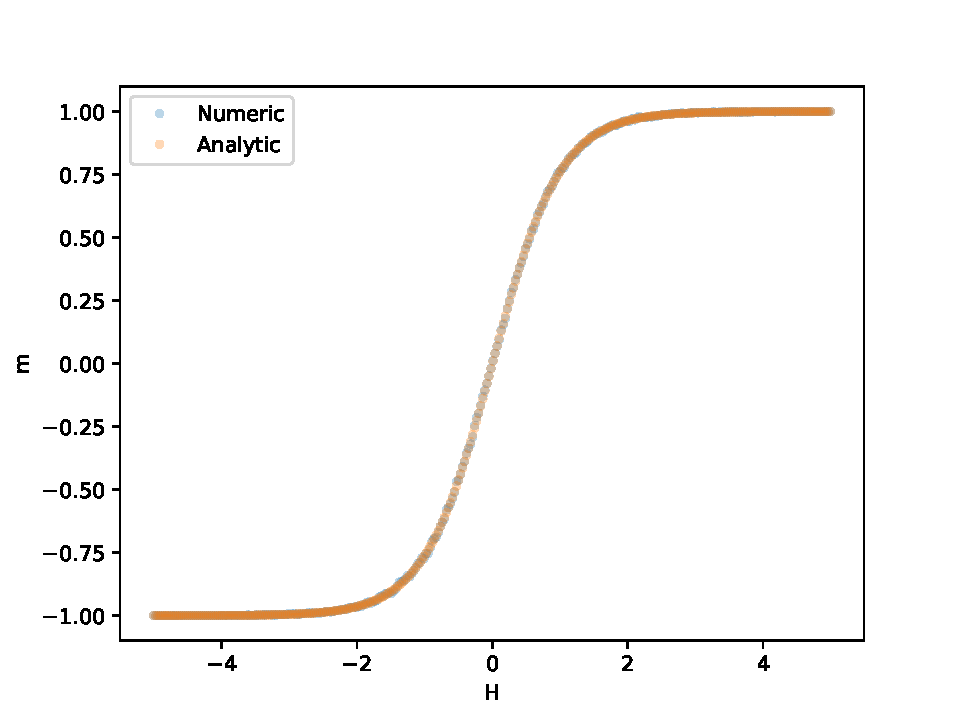
\includegraphics[width=.9\textwidth]{images/Ex1_Graph.pdf}
    \caption{Magnetisierung $m$ in Abhängigkeit des äußeren Magnetfeldes $H$.}
\end{figure}
\begin{figure}
    \centering
    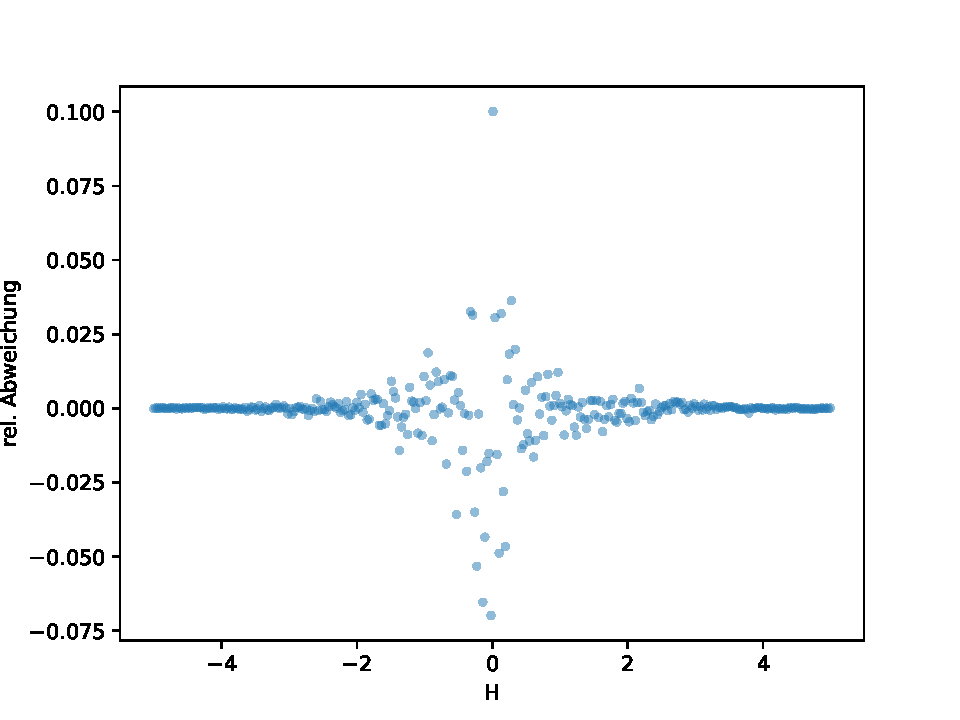
\includegraphics[width=.9\textwidth]{images/Ex1_Abweichung.pdf}
    \caption{Rel. Abweichung zwischen der numerischen und der analytischen Magnetisierung.}
\end{figure}



\subsection{Aufgabe 2} 
\subsubsection{1.}

In den Abbildungen sind Momentaufnahmen der Spins dargestellt. 
Bei $k_BT = 1$ sind zu Anfang noch größere Bereiche von gleich ausgerichteten Spins zu erkennen.
Nach weiteren Sweeps stellen sich aber alle Spins in eine Richtung.
Bei einem anderen Durchlauf sind nicht alle, sondern nur jeweils in drei großen getrennten Bereichen die Spins gleich ausgerichtet. 
Bei $k_BT = 3$ befindet sich das System in einer anderen Phase. 
Es sind keine größeren Bereiche homogener Spinausrichtung mehr zu erkennen.
\begin{figure}
    \centering
    \begin{subfigure}{0.45\textwidth}
      \centering
      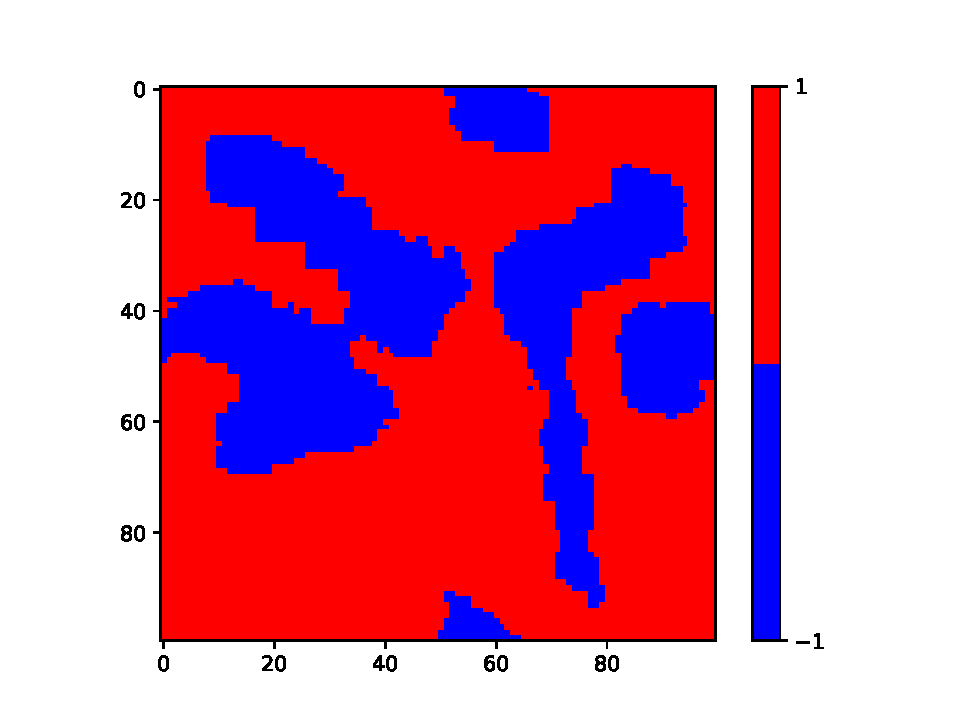
\includegraphics[width=\linewidth]{images/Ising1_0.pdf}
      \caption{Snapshot 1}
      \label{fig:image1}
    \end{subfigure}
    \hfill
    \begin{subfigure}{0.45\textwidth}
      \centering
      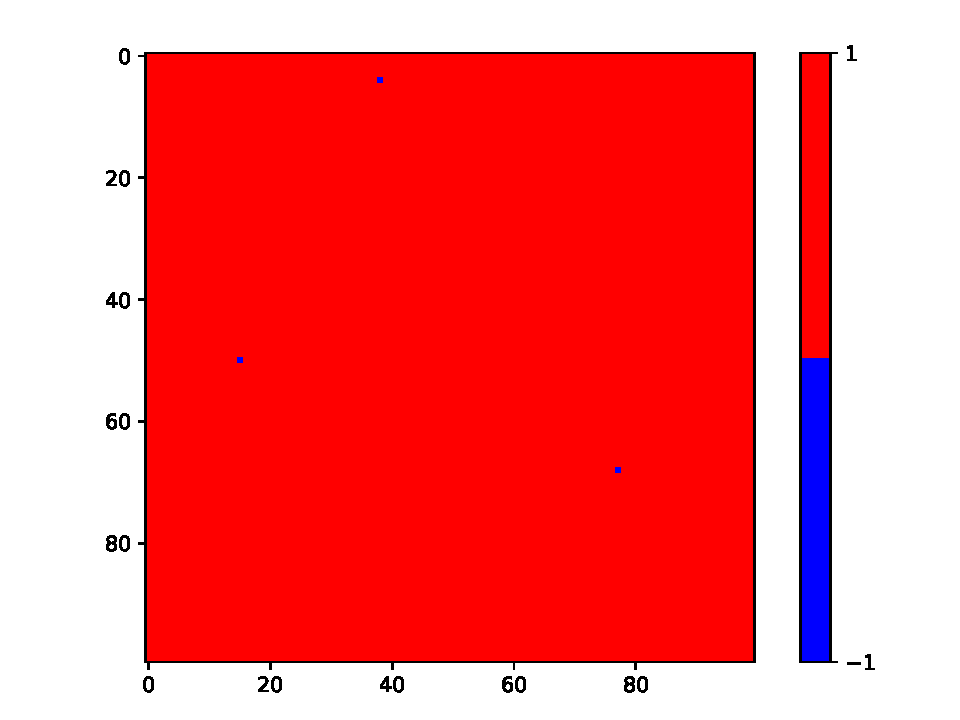
\includegraphics[width=\linewidth]{images/Ising1_2.pdf}
      \caption{Snapshot 2}
      \label{fig:image2}
    \end{subfigure}
    
    \vspace{0.5cm}
    
    \begin{subfigure}{0.45\textwidth}
      \centering
      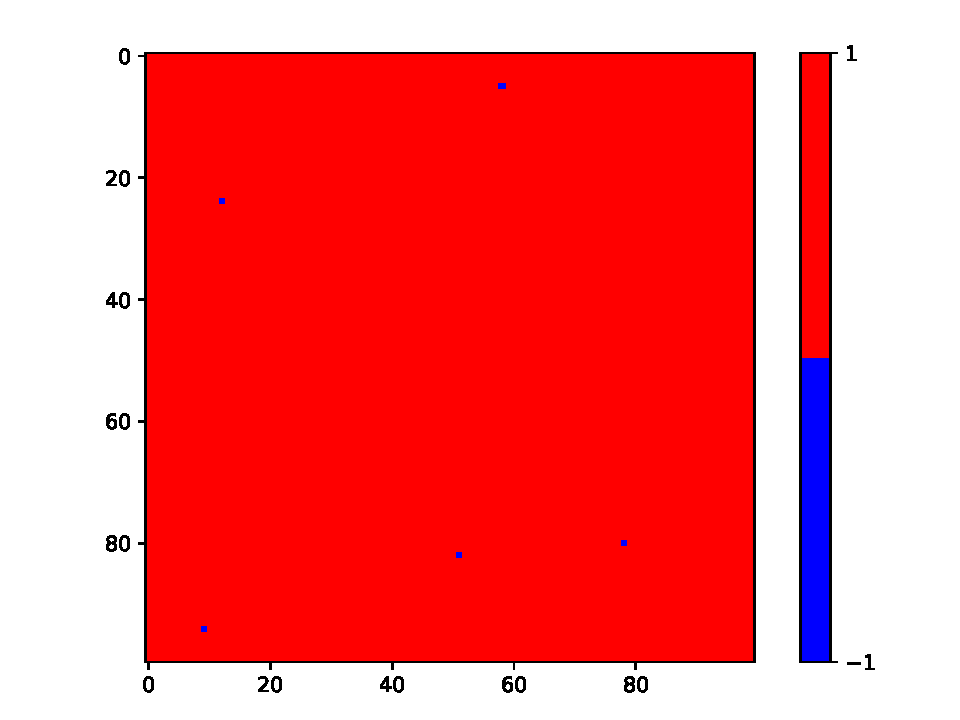
\includegraphics[width=\linewidth]{images/Ising1_3.pdf}
      \caption{Snapshot 3}
      \label{fig:image3}
    \end{subfigure}
    \hfill
    \begin{subfigure}{0.45\textwidth}
      \centering
      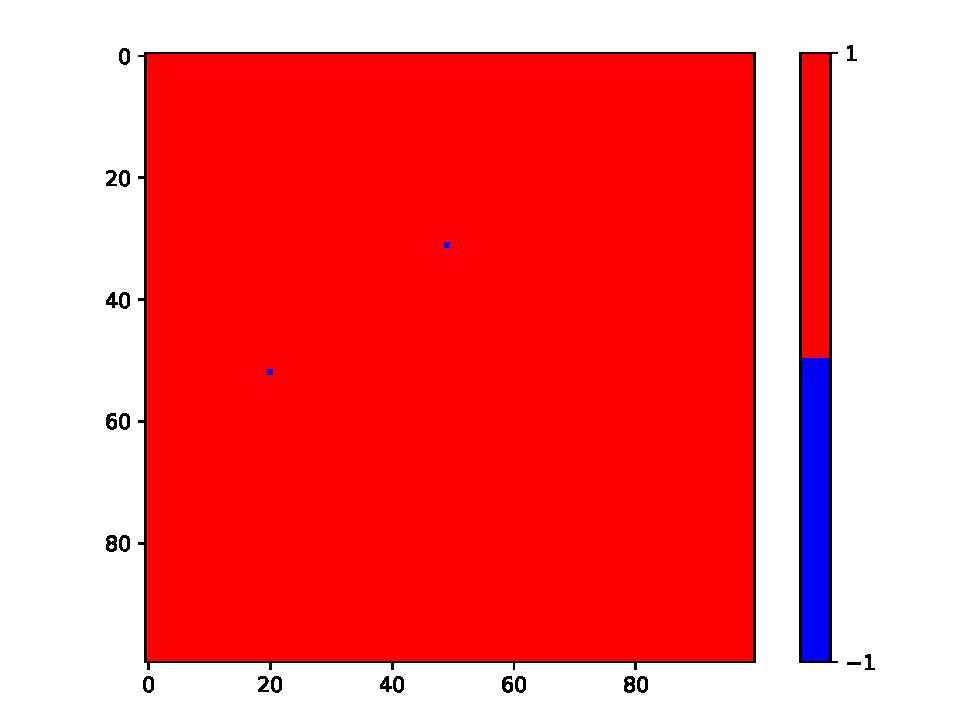
\includegraphics[width=\linewidth]{images/Ising1_4.pdf}
      \caption{Snapshot 4}
      \label{fig:image4}
    \end{subfigure}
    \caption{Durchlauf 1 mit $k_BT = 1$}
    \label{fig:two_by_two}
  \end{figure}

  \begin{figure}
    \centering
    \begin{subfigure}{0.45\textwidth}
      \centering
      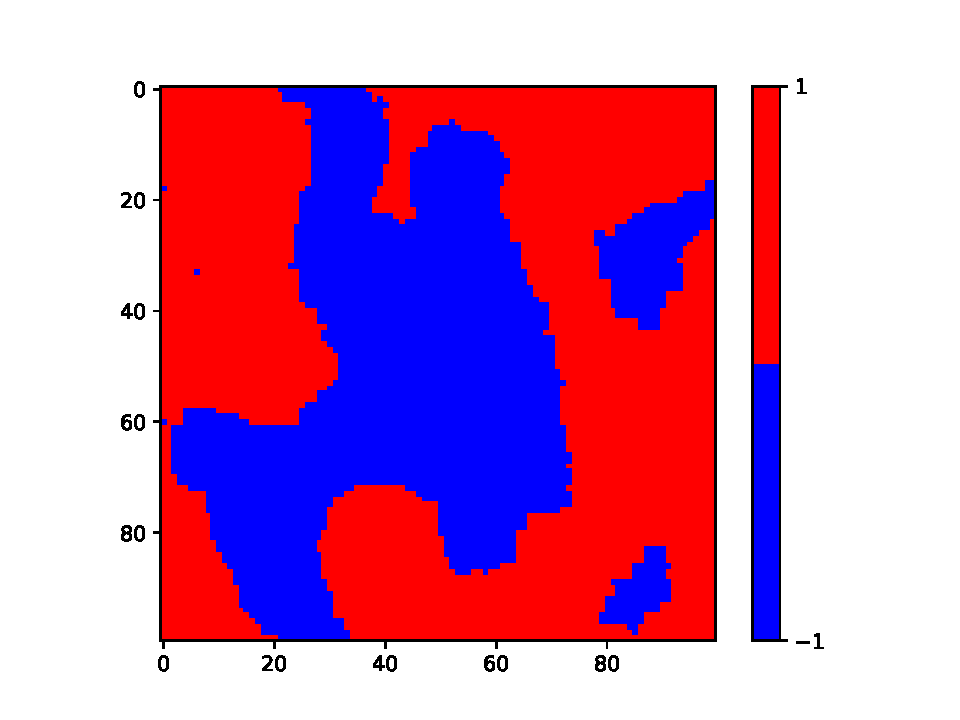
\includegraphics[width=\linewidth]{images/Ising1_0_copy.pdf}
      \caption{Snapshot 1}
      \label{fig:image1}
    \end{subfigure}
    \hfill
    \begin{subfigure}{0.45\textwidth}
      \centering
      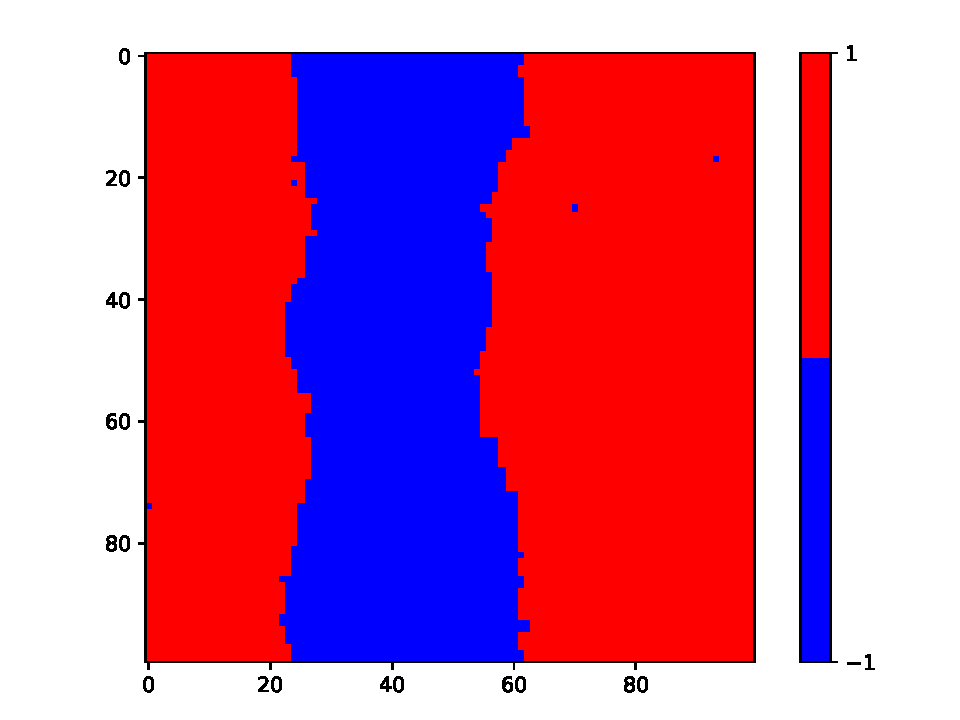
\includegraphics[width=\linewidth]{images/Ising1_2_copy.pdf}
      \caption{Snapshot 2}
      \label{fig:image2}
    \end{subfigure}
    
    \vspace{0.5cm}
    
    \begin{subfigure}{0.45\textwidth}
      \centering
      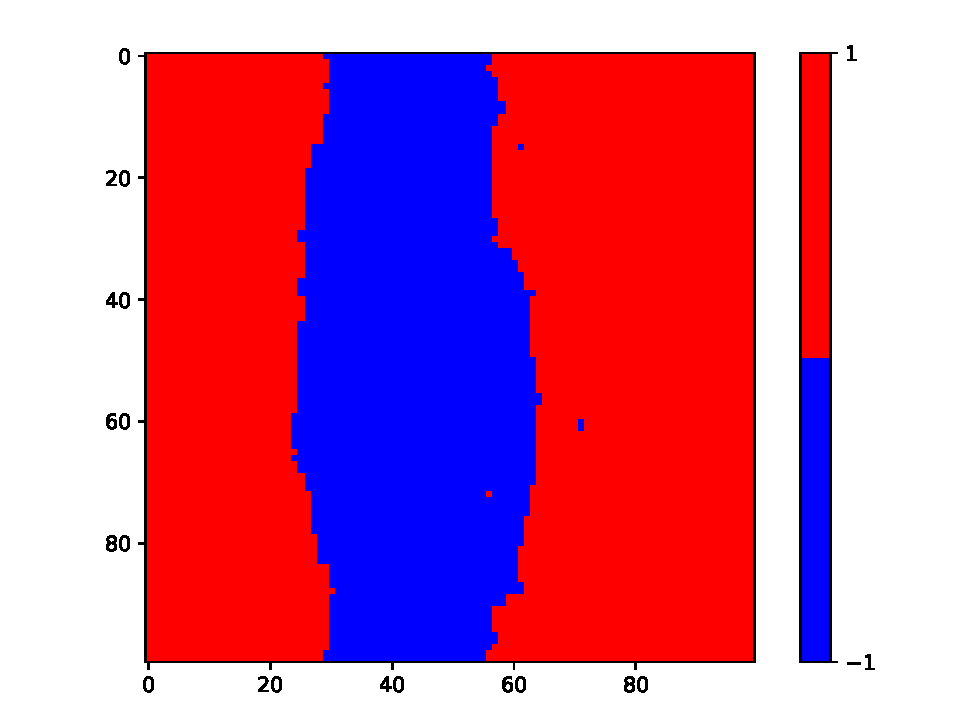
\includegraphics[width=\linewidth]{images/Ising1_3_copy.pdf}
      \caption{Snapshot 3}
      \label{fig:image3}
    \end{subfigure}
    \hfill
    \begin{subfigure}{0.45\textwidth}
      \centering
      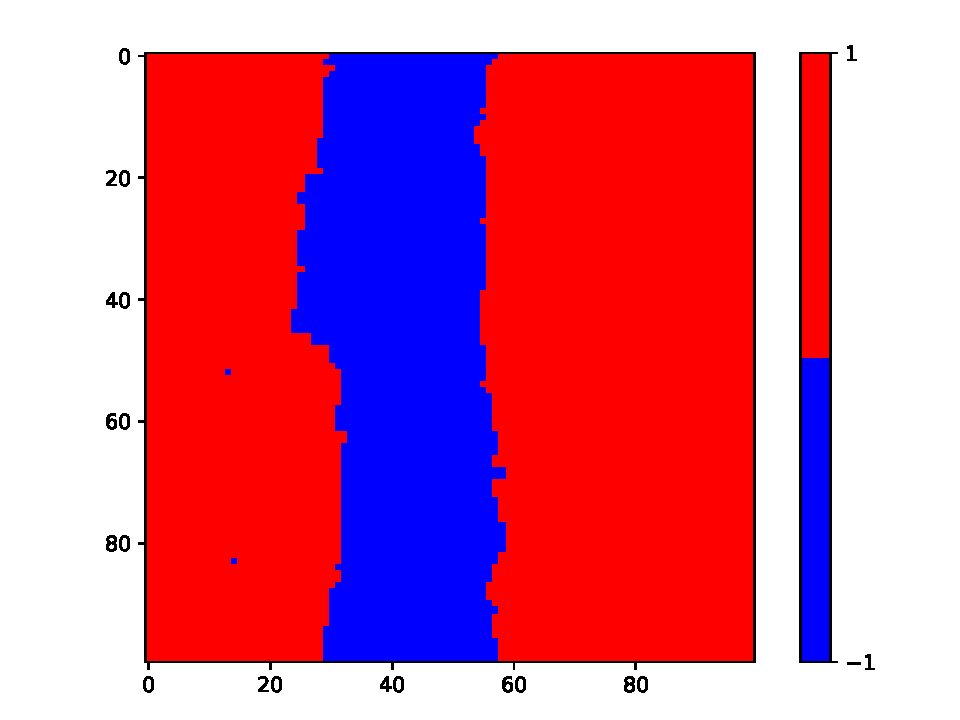
\includegraphics[width=\linewidth]{images/Ising1_4_copy.pdf}
      \caption{Snapshot 4}
      \label{fig:image4}
    \end{subfigure}
    \caption{Durchlauf 2 mit $k_BT = 1$}
    \label{fig:two_by_two}
  \end{figure}

  \begin{figure}
    \centering
    \begin{subfigure}{0.45\textwidth}
      \centering
      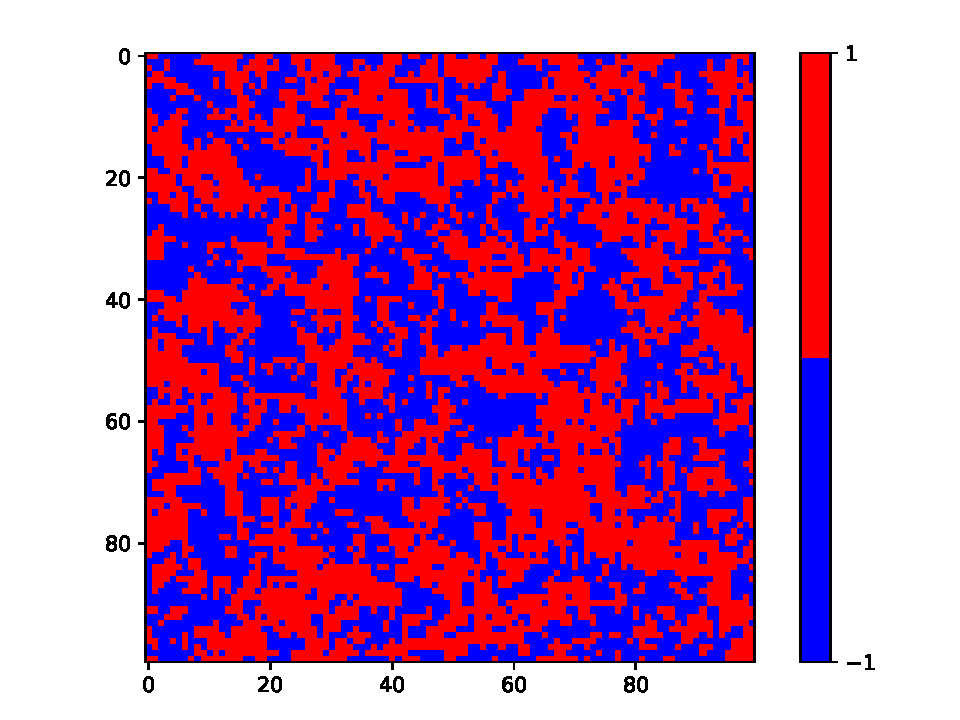
\includegraphics[width=\linewidth]{images/Ising3_0.pdf}
      \caption{Snapshot 1}
      \label{fig:image1}
    \end{subfigure}
    \hfill
    \begin{subfigure}{0.45\textwidth}
      \centering
      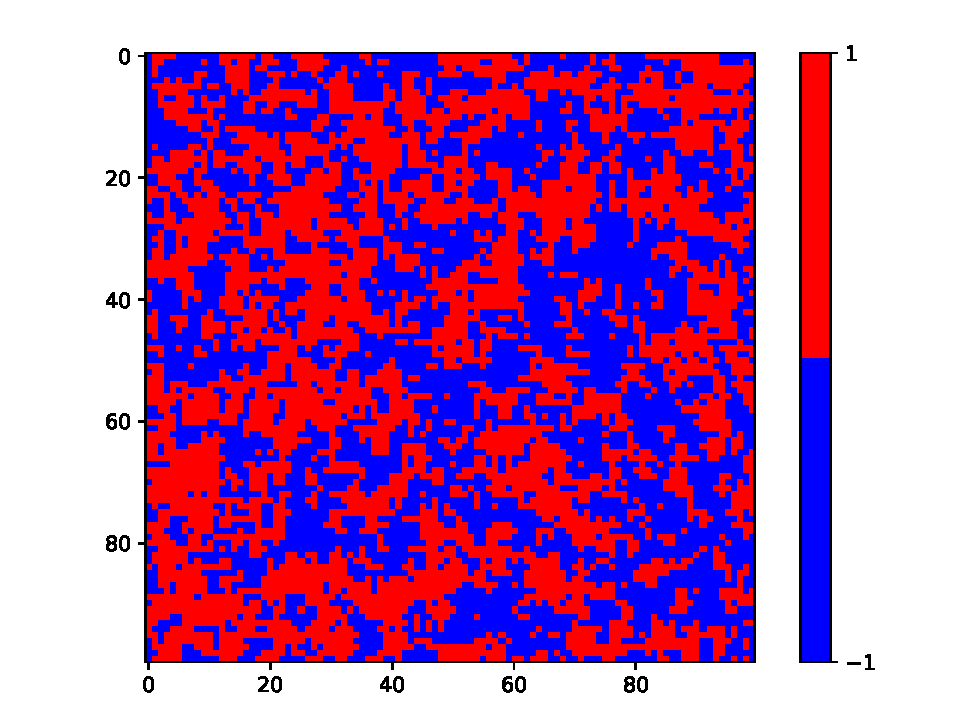
\includegraphics[width=\linewidth]{images/Ising3_2.pdf}
      \caption{Snapshot 2}
      \label{fig:image2}
    \end{subfigure}
    
    \vspace{0.5cm}
    
    \begin{subfigure}{0.45\textwidth}
      \centering
      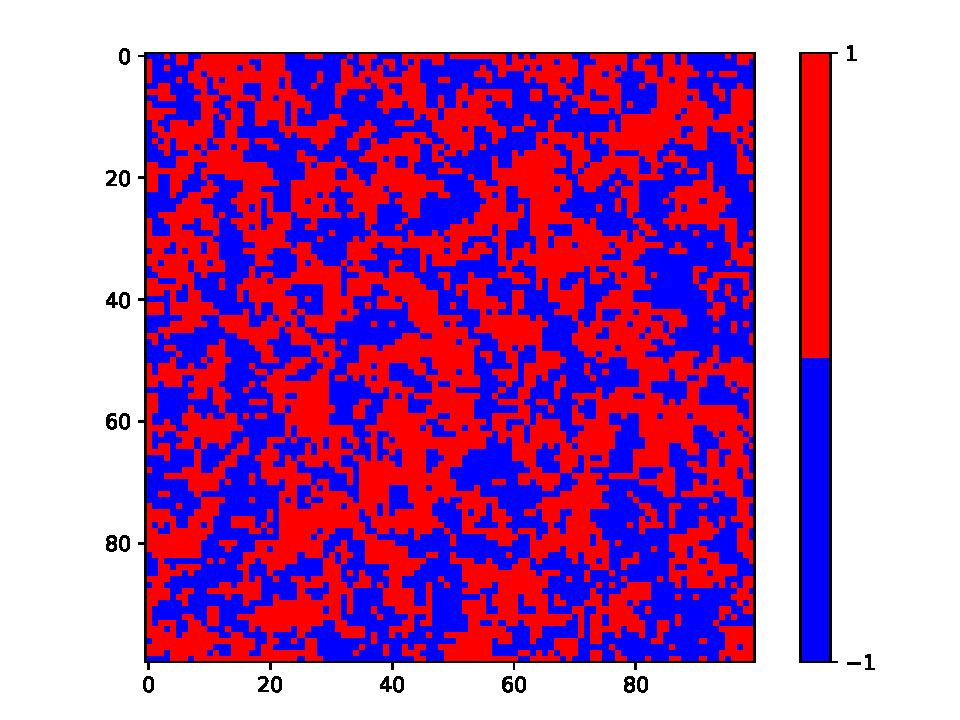
\includegraphics[width=\linewidth]{images/Ising3_3.pdf}
      \caption{Snapshot 3}
      \label{fig:image3}
    \end{subfigure}
    \hfill
    \begin{subfigure}{0.45\textwidth}
      \centering
      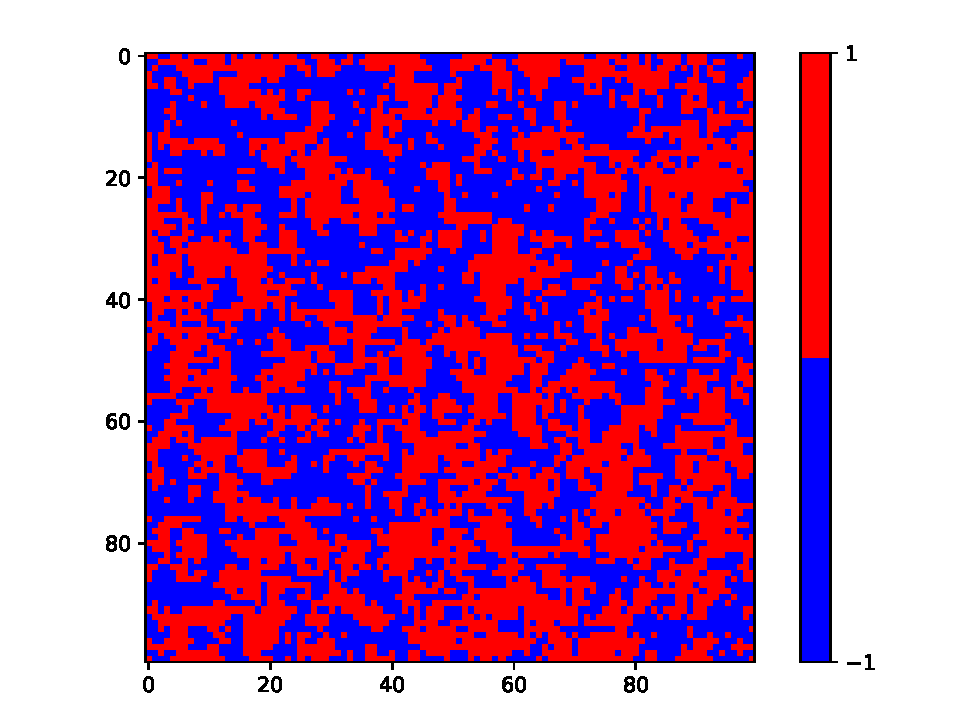
\includegraphics[width=\linewidth]{images/Ising3_4.pdf}
      \caption{Snapshot 4}
      \label{fig:image4}
    \end{subfigure}
    \caption{$k_BT = 3$}
    \label{fig:two_by_two}
  \end{figure}


  \subsubsection{2.}

  Es wird die mittlere Energie bestimmt. Dazu wird die Energie über alle Moves eines Sweeps gemittelt. 
  Für die mittlere Energie pro Spin wird diese Energie wird dann durch die Anzahl Spins geteilt.
  Trotz verschiedener Anfangsverteilungen nähert sich bei hoher Temperaturen diese mittlere Energy pro Spin jeweils einem ähnlich Wert an.
  Bei kleinen Temperaturen dauert diese Annäherung länger. 
  Je nach Durchlauf variiert diese Anzahl notwendiger Sweeps. Bei den meisten Durchläufen ist das System spätestens nach ca. 5000 Sweeps auch bei der niedrigen Temperatur warm gelaufen.
  \begin{figure}
    \centering
    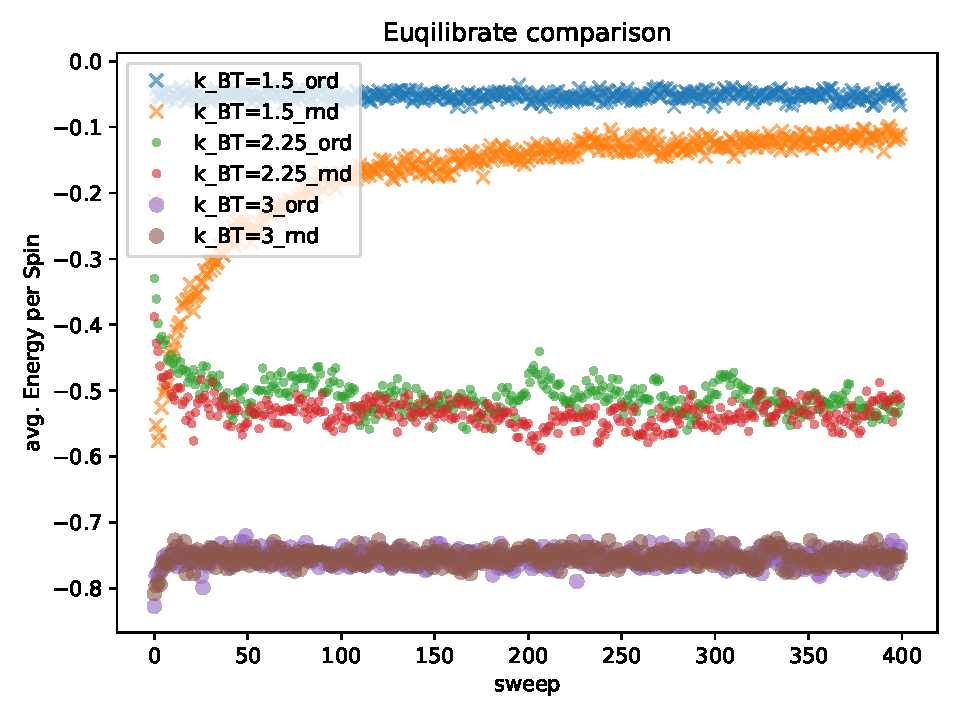
\includegraphics[width=.9\textwidth]{images/av_energy2.pdf}
    \caption{Mittlere Energie pro Spin in Abhängigkeit der Anzahl sweeps. Es wird eine geordnete mit einer zufälligen Anfangsverteilung der Spins verglichen. Hier im Bereiche von 400 Sweeps.}
  \end{figure}
  \begin{figure}
    \centering
    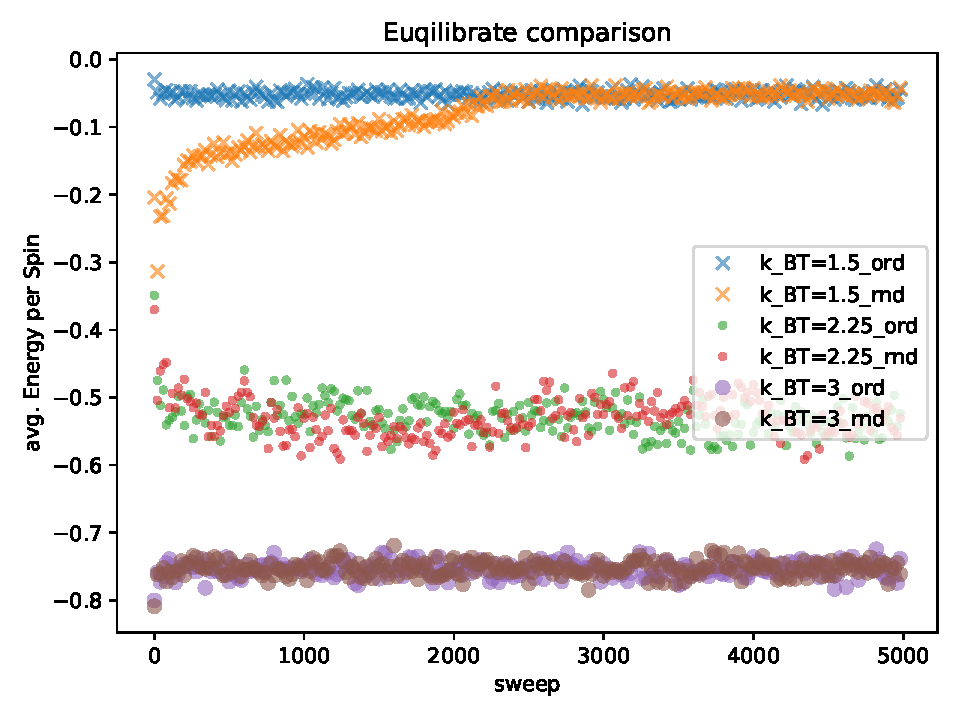
\includegraphics[width=.9\textwidth]{images/av_energy3.pdf}
    \caption{Mittlere Energie pro Spin in Abhängigkeit der Anzahl sweeps. Es wird eine geordnete mit einer zufälligen Anfangsverteilung der Spins verglichen. Hier im Bereiche von 5000 Sweeps.}
  \end{figure}
